%%%%%%%%%%%%  Generated using docx2latex.com  %%%%%%%%%%%%%%

%%%%%%%%%%%%  v2.0.0-beta  %%%%%%%%%%%%%%

\documentclass[a4paper,12pt]{article}

% Other options in place of 'report' are 1)article 2)book 3)letter
% Other options in place of 'a4paper' are 1)a5paper 2)b5paper 3)letterpaper 4)legalpaper 5)executivepaper


 %%%%%%%%%%%%  Include Packages  %%%%%%%%%%%%%%


\usepackage{amsmath}
\usepackage{latexsym}
\usepackage{amsfonts}
\usepackage[normalem]{ulem}
\usepackage{array}
\usepackage{amssymb}
\usepackage{graphicx}
\usepackage{subfig}
\usepackage{wrapfig}
\usepackage{wasysym}
\usepackage{enumitem}
\usepackage{adjustbox}
\usepackage{ragged2e}
\usepackage{longtable}
\usepackage{changepage}
\usepackage{setspace}
\usepackage{hhline}
\usepackage{multicol}
\usepackage{float}
\usepackage{multirow}
\usepackage{makecell}
\usepackage{fancyhdr}
\usepackage[toc,page]{appendix}
\usepackage[a4paper,left=0.79in,right=0.79in,top=0.79in,bottom=0.79in,headheight=1in]{geometry}
\usepackage[utf8]{inputenc}
\usepackage[T1]{fontenc}
\usepackage{color,hyperref}
\definecolor{darkblue}{rgb}{0.0,0.0,1}


 %%%%%%%%%%%%  Define Colors For Hyperlinks  %%%%%%%%%%%%%%


\urlstyle{same}


 %%%%%%%%%%%%  Set Depths for Sections  %%%%%%%%%%%%%%

% 1) Section
% 1.1) SubSection
% 1.1.1) SubSubSection
% 1.1.1.1) Paragraph
% 1.1.1.1.1) Subparagraph


\setcounter{tocdepth}{5}
\setcounter{secnumdepth}{5}


 %%%%%%%%%%%%  Set Page Margins  %%%%%%%%%%%%%%


\everymath{\displaystyle}


 %%%%%%%%%%%%  Set Depths for Nested Lists created by \begin{enumerate}  %%%%%%%%%%%%%%


\setlistdepth{9}
\newlist{custom_Enumerate}{enumerate}{9}
	\setlist[custom_Enumerate,1]{label=\arabic*)}
	\setlist[custom_Enumerate,2]{label=\alph*)}
	\setlist[custom_Enumerate,3]{label=(\roman*)}
	\setlist[custom_Enumerate,4]{label=(\arabic*)}
	\setlist[custom_Enumerate,5]{label=(\Alph*)}
	\setlist[custom_Enumerate,6]{label=(\Roman*)}
	\setlist[custom_Enumerate,7]{label=\arabic*}
	\setlist[custom_Enumerate,8]{label=\alph*}
	\setlist[custom_Enumerate,9]{label=\roman*}

\renewlist{itemize}{itemize}{9}
	\setlist[itemize]{label=$\cdot$}
	\setlist[itemize,1]{label=\textbullet}
	\setlist[itemize,2]{label=$\circ$}
	\setlist[itemize,3]{label=$\ast$}
	\setlist[itemize,4]{label=$\dagger$}
	\setlist[itemize,5]{label=$\triangleright$}
	\setlist[itemize,6]{label=$\bigstar$}
	\setlist[itemize,7]{label=$\blacklozenge$}
	\setlist[itemize,8]{label=$\prime$}



\begin{document}
\sloppy
\begin{FlushLeft}
{\fontsize{12pt}{12pt}\selectfont {\fontsize{24pt}{24pt}\selectfont \hspace*{0.5in}Introduction to Compiler Design Project1 Report}}
\end{FlushLeft}\par

\begin{FlushLeft}
{\fontsize{12pt}{12pt}\selectfont {\fontsize{24pt}{24pt}\selectfont 0416324胡安鳳}}
\end{FlushLeft}\par

\begin{FlushLeft}
{\fontsize{12pt}{12pt}\selectfont \begin{FlushLeft}
{\fontsize{20pt}{20pt}\selectfont 1.Programming platform: }}
\end{FlushLeft}\par

\begin{FlushLeft}
{\fontsize{12pt}{12pt}\selectfont \begin{FlushLeft}
{\fontsize{14pt}{14pt}\selectfont Ubuntu 16.04 x64 with lex, gcc and c language.}}
\end{FlushLeft}\par



%%%%%%%%%%%%%%%%%%%% Figure/Image No: 1 starts here %%%%%%%%%%%%%%%%%%%%

\begin{figure}[H]
	\begin{FlushLeft}
		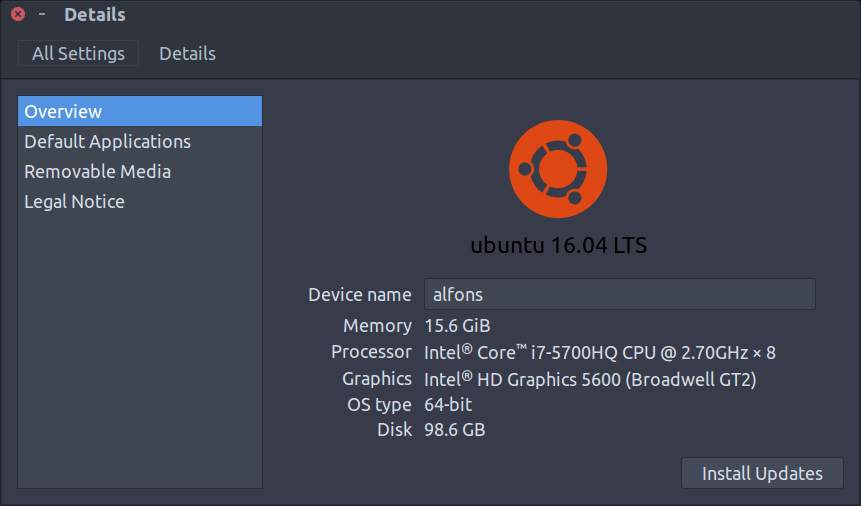
\includegraphics[width=3.59in,height=2.11in]{./media/image1.png}
	\end{FlushLeft}\end{figure}


%%%%%%%%%%%%%%%%%%%% Figure/Image No: 1 Ends here %%%%%%%%%%%%%%%%%%%%

\begin{FlushLeft}
{\fontsize{12pt}{12pt}\selectfont \begin{FlushLeft}
}
\end{FlushLeft}
\vspace{12pt}\begin{FlushLeft}
{\fontsize{12pt}{12pt}\selectfont \begin{FlushLeft}
{\fontsize{20pt}{20pt}\selectfont 2.Lex scanner ability}}
\end{FlushLeft}\par

\begin{FlushLeft}
{\fontsize{12pt}{12pt}\selectfont \begin{FlushLeft}
{\fontsize{14pt}{14pt}\selectfont Able to detect the necessary elements including.}}
\end{FlushLeft}\par

\begin{FlushLeft}
{\fontsize{12pt}{12pt}\selectfont \begin{FlushLeft}
{\fontsize{14pt}{14pt}\selectfont (1) Delimiters}}
\end{FlushLeft}\par

\begin{FlushLeft}
{\fontsize{12pt}{12pt}\selectfont \begin{FlushLeft}
{\fontsize{14pt}{14pt}\selectfont (2) Arithmetic, Relational, and Logical Operators}}
\end{FlushLeft}\par

\begin{FlushLeft}
{\fontsize{12pt}{12pt}\selectfont \begin{FlushLeft}
{\fontsize{14pt}{14pt}\selectfont (3) Keywords}}
\end{FlushLeft}\par

\begin{FlushLeft}
{\fontsize{12pt}{12pt}\selectfont \begin{FlushLeft}
{\fontsize{14pt}{14pt}\selectfont (4) Identifiers}}
\end{FlushLeft}\par

\begin{FlushLeft}
{\fontsize{12pt}{12pt}\selectfont \begin{FlushLeft}
{\fontsize{14pt}{14pt}\selectfont (5) Integer Constants}}
\end{FlushLeft}\par

\begin{FlushLeft}
{\fontsize{12pt}{12pt}\selectfont \begin{FlushLeft}
{\fontsize{14pt}{14pt}\selectfont (6) Scientific Notations}}
\end{FlushLeft}\par

\begin{FlushLeft}
{\fontsize{12pt}{12pt}\selectfont \begin{FlushLeft}
{\fontsize{14pt}{14pt}\selectfont (7) Floating-point Constants\hspace*{0.49in}}}
\end{FlushLeft}\par

\begin{FlushLeft}
{\fontsize{12pt}{12pt}\selectfont \begin{FlushLeft}
{\fontsize{14pt}{14pt}\selectfont (8) String Constants}}
\end{FlushLeft}\par

\begin{FlushLeft}
{\fontsize{12pt}{12pt}\selectfont \begin{FlushLeft}
{\fontsize{14pt}{14pt}\selectfont (9) Control character [$\textbackslash$n]}}
\end{FlushLeft}\par

\begin{FlushLeft}
{\fontsize{12pt}{12pt}\selectfont \begin{FlushLeft}
{\fontsize{14pt}{14pt}\selectfont Able to discard the unnecessary elements, but still to the necessary processing}}
\end{FlushLeft}\par

\begin{FlushLeft}
{\fontsize{12pt}{12pt}\selectfont \begin{FlushLeft}
{\fontsize{14pt}{14pt}\selectfont (1) Whitespace and tab[$\textbackslash$r]}}
\end{FlushLeft}\par

\begin{FlushLeft}
{\fontsize{12pt}{12pt}\selectfont \begin{FlushLeft}
{\fontsize{14pt}{14pt}\selectfont \hspace*{0.49in}Use the LIST function in lex template to do the source code indentation}}
\end{FlushLeft}\par

\begin{FlushLeft}
{\fontsize{12pt}{12pt}\selectfont \begin{FlushLeft}
{\fontsize{14pt}{14pt}\selectfont \hspace*{0.49in}correctly}}
\end{FlushLeft}\par

\begin{FlushLeft}
{\fontsize{12pt}{12pt}\selectfont \begin{FlushLeft}
{\fontsize{14pt}{14pt}\selectfont (2) Comments}}
\end{FlushLeft}\par

\begin{FlushLeft}
{\fontsize{12pt}{12pt}\selectfont \begin{FlushLeft}
{\fontsize{14pt}{14pt}\selectfont \hspace*{0.49in}Detecting the following two types of comments and specify the illegal \hspace*{0.49in}comments.}}
\end{FlushLeft}\par

\begin{FlushLeft}
{\fontsize{12pt}{12pt}\selectfont \begin{FlushLeft}
{\fontsize{14pt}{14pt}\selectfont \hspace*{0.49in}e.g. /*This is a comment */ is a legal c style comment}}
\end{FlushLeft}\par

\begin{FlushLeft}
{\fontsize{12pt}{12pt}\selectfont \begin{FlushLeft}
\hspace*{0.49in}{\fontsize{14pt}{14pt}\selectfont /* this is a comment // line with some /* and}}
\end{FlushLeft}\par

\begin{FlushLeft}
{\fontsize{12pt}{12pt}\selectfont \begin{FlushLeft}
{\fontsize{14pt}{14pt}\selectfont ~~~ \hspace*{0.49in}// delimiters */ is also a legal c style comment}}
\end{FlushLeft}\par

\begin{FlushLeft}
{\fontsize{12pt}{12pt}\selectfont \begin{FlushLeft}
{\fontsize{14pt}{14pt}\selectfont \hspace*{0.49in}However, /*this~is a tricky comment*/  this part is not considered to be a \hspace*{0.49in}comment but some identifiers*/ is not a legal comment (the part between */ \hspace*{0.49in}and */ is not the part of c style comment}}
\end{FlushLeft}\par

\begin{FlushLeft}
{\fontsize{12pt}{12pt}\selectfont \begin{FlushLeft}
{\fontsize{14pt}{14pt}\selectfont \hspace*{0.49in}// this is a comment // line */ /* with some /* delimiters */ before the end is a \hspace*{0.49in}legal c style comments}}
\end{FlushLeft}\par

\begin{FlushLeft}
{\fontsize{12pt}{12pt}\selectfont \begin{FlushLeft}
{\fontsize{14pt}{14pt}\selectfont (3) Pseudocomments}}
\end{FlushLeft}\par

\begin{FlushLeft}
{\fontsize{12pt}{12pt}\selectfont \begin{FlushLeft}
{\fontsize{14pt}{14pt}\selectfont \hspace*{0.49in}Detect and use them to activate/deactive the function in lex scanner.}}
\end{FlushLeft}\par

\begin{FlushLeft}
{\fontsize{12pt}{12pt}\selectfont \begin{FlushLeft}
{\fontsize{14pt}{14pt}\selectfont I use the following tricky testcase to test my scanner.}}
\end{FlushLeft}\par

\begin{FlushLeft}
{\fontsize{12pt}{12pt}\selectfont \begin{FlushLeft}
{\fontsize{14pt}{14pt}\selectfont Testcase is at: \href{https://pastebin.com/83zRkxmB}{https://pastebin.com/83zRkxmB}}}
\end{FlushLeft}\par

\begin{FlushLeft}
{\fontsize{12pt}{12pt}\selectfont \begin{FlushLeft}
{\fontsize{14pt}{14pt}\selectfont Output result is at: \href{https://pastebin.com/ujCEJ0CB}{https://pastebin.com/ujCEJ0CB}}}
\end{FlushLeft}\par

\begin{FlushLeft}
{\fontsize{12pt}{12pt}\selectfont \begin{FlushLeft}
{\fontsize{14pt}{14pt}\selectfont (The lextemplate has been modified to fully detect all the bad characters, which will loop till the end to detect any illegal characters not specified in the project requirements and specify the C and C++ style comments respectively)}}
\end{FlushLeft}\par

\begin{FlushLeft}
{\fontsize{12pt}{12pt}\selectfont \begin{FlushLeft}
{\fontsize{14pt}{14pt}\selectfont Lextemplate~is able to specify the hardest part: delimiting two comments /*c1*/  /*c2*/ modified from the regex of only [/][.](.$ \vert $[$\textbackslash$n])[/][*] which will specify only one comment since lex uses greedy method(or say greedy algorithm), the modified regex should be }}
\end{FlushLeft}\par

\begin{FlushLeft}
{\fontsize{12pt}{12pt}\selectfont \begin{FlushLeft}
{\fontsize{14pt}{14pt}\selectfont [/][*]([$ \string^ $*]$ \vert $[$\textbackslash$n]$ \vert $[*]+[$ \string^ $/]$ \vert $[/][*])*[*]+[/] which means }}
\end{FlushLeft}\par

\begin{FlushLeft}
{\fontsize{12pt}{12pt}\selectfont \begin{FlushLeft}
{\fontsize{14pt}{14pt}\selectfont (1) We may not permit the star symbol in the middle (or we may, but the star symbol CANNOT BE FOLLOWED BY THE SLASH since the slash symbol only appears at the end of the comments.}}
\end{FlushLeft}\par

\begin{FlushLeft}
{\fontsize{12pt}{12pt}\selectfont \begin{FlushLeft}
{\fontsize{14pt}{14pt}\selectfont (2) The $\textbackslash$n new line symbol is legal in the c style comment}}
\end{FlushLeft}\par

\begin{FlushLeft}
{\fontsize{12pt}{12pt}\selectfont \begin{FlushLeft}
{\fontsize{14pt}{14pt}\selectfont (3) If the star symbol has to be appeared in the comment, then there should be no / (slash symbol) after it, since */ should only appear in the end of the comment.}}
\end{FlushLeft}\par

\begin{FlushLeft}
{\fontsize{12pt}{12pt}\selectfont \begin{FlushLeft}
{\fontsize{14pt}{14pt}\selectfont (4) The /* in the symbol is acceptable just as the problem defined in the project pdf}}
\end{FlushLeft}\par

\begin{FlushLeft}
{\fontsize{12pt}{12pt}\selectfont \begin{FlushLeft}
{\fontsize{14pt}{14pt}\selectfont Also it can detect the wrong style of comment such as /**/xxx */ the xxx part should be specified as identifier, delimiter or relational, arithmetical operator.}}
\end{FlushLeft}\par

\begin{FlushLeft}
{\fontsize{12pt}{12pt}\selectfont \begin{FlushLeft}
{\fontsize{14pt}{14pt}\selectfont (5) [*]+ at the end before / to accept multi star symbol before the slash such as }}
\end{FlushLeft}\par

\begin{FlushLeft}
{\fontsize{12pt}{12pt}\selectfont \begin{FlushLeft}
{\fontsize{14pt}{14pt}\selectfont /*wfiuhwef/*piuhwefiu*****/~ is still a legal C style comment.}}
\end{FlushLeft}\par

\begin{FlushLeft}
{\fontsize{12pt}{12pt}\selectfont \begin{FlushLeft}
{\fontsize{14pt}{14pt}\selectfont For the other illegal elements that need to be specified out and terminated.}}
\end{FlushLeft}\par

\begin{FlushLeft}
{\fontsize{12pt}{12pt}\selectfont \begin{FlushLeft}
{\fontsize{14pt}{14pt}\selectfont Such~as 9$"$9 or $"$999  $"$9$"$9$"$$"$9 and 9999$\&$@$\#$@!$\$$$\#$@(these symbols are not considered to be the delimiters), lots of trash like them should be detected and generate error message.}}
\end{FlushLeft}\par

\begin{FlushLeft}
{\fontsize{12pt}{12pt}\selectfont \begin{FlushLeft}
{\fontsize{14pt}{14pt}\selectfont Use regex ["]?([0-9]+["])+ once a $"$ append with integer or a integer cross-appearing with an $"$ are both illegal. (consider the $"$999$"$ is still legal since it is a string)}}
\end{FlushLeft}\par

\begin{FlushLeft}
{\fontsize{12pt}{12pt}\selectfont \begin{FlushLeft}
{\fontsize{14pt}{14pt}\selectfont Or such identifier like 9ast 88you 100$ \_ $int is not legal.}}
\end{FlushLeft}\par

\begin{FlushLeft}
{\fontsize{12pt}{12pt}\selectfont \begin{FlushLeft}
{\fontsize{14pt}{14pt}\selectfont Use regex [0-9]+[a-zA-Z$ \_ $] to identify an illegal identifier}}
\end{FlushLeft}\par

\begin{FlushLeft}
{\fontsize{12pt}{12pt}\selectfont \begin{FlushLeft}
{\fontsize{14pt}{14pt}\selectfont And the rest like *$\&$$ \string^ $(*$\&$$ \string^ $ trash should be treated as the lowest precedence and use . (dot symbol or say the rest) after all the rule are exhausted.}}
\end{FlushLeft}\par

\begin{FlushLeft}
{\fontsize{12pt}{12pt}\selectfont \begin{FlushLeft}
{\fontsize{14pt}{14pt}\selectfont For pesudocomments , they all have the same form }}
\end{FlushLeft}\par

\begin{FlushLeft}
{\fontsize{12pt}{12pt}\selectfont \begin{FlushLeft}
{\fontsize{14pt}{14pt}\selectfont "//$\&$S-"(.)*[$\textbackslash$n]}}
\end{FlushLeft}\par

\begin{FlushLeft}
{\fontsize{12pt}{12pt}\selectfont \begin{FlushLeft}
{\fontsize{14pt}{14pt}\selectfont and once encountered, do the necessary modification of option and line$ \_ $num++ to count it as a whole line.}}
\end{FlushLeft}\par

\begin{FlushLeft}
{\fontsize{12pt}{12pt}\selectfont \begin{FlushLeft}
{\fontsize{20pt}{20pt}\selectfont 3. How to build and run the program}}
\end{FlushLeft}\par

\begin{FlushLeft}
{\fontsize{12pt}{12pt}\selectfont \begin{FlushLeft}
{\fontsize{14pt}{14pt}\selectfont Using the makefile in Linux and aggregate all the necessary compilation altogether.}}
\end{FlushLeft}\par

\begin{FlushLeft}
{\fontsize{12pt}{12pt}\selectfont \begin{FlushLeft}
{\fontsize{14pt}{14pt}\selectfont (1) Use lex to generate lex.yy.c from the source code of lextemplate}}
\end{FlushLeft}\par

\begin{FlushLeft}
{\fontsize{12pt}{12pt}\selectfont \begin{FlushLeft}
{\fontsize{14pt}{14pt}\selectfont $\$$ lex lextemplate.l }}
\end{FlushLeft}\par

\begin{FlushLeft}
{\fontsize{12pt}{12pt}\selectfont \begin{FlushLeft}
{\fontsize{14pt}{14pt}\selectfont (2) Gcc it, -lfl tells gcc to use the lex(or flex) library}}
\end{FlushLeft}\par

\begin{FlushLeft}
{\fontsize{12pt}{12pt}\selectfont \begin{FlushLeft}
{\fontsize{14pt}{14pt}\selectfont $\$$ gcc -o scanner lex.yy.c -lfl}}
\end{FlushLeft}\par

\begin{FlushLeft}
{\fontsize{12pt}{12pt}\selectfont \begin{FlushLeft}
{\fontsize{14pt}{14pt}\selectfont (3) Run it (file in the same path folder)}}
\end{FlushLeft}\par

\begin{FlushLeft}
{\fontsize{12pt}{12pt}\selectfont \begin{FlushLeft}
{\fontsize{14pt}{14pt}\selectfont $\$$ ./scanner [filename]}}
\end{FlushLeft}\par

\end{document}